
\subsection{Output characteristic}
Some simulations have been made in order to make sure the circuits works as expected. First we computed the curves for a series of moving pulses as it could be in a practical case. Hereafter are the curves obtained in normal operation conditions. 
\begin{figure}[!ht]
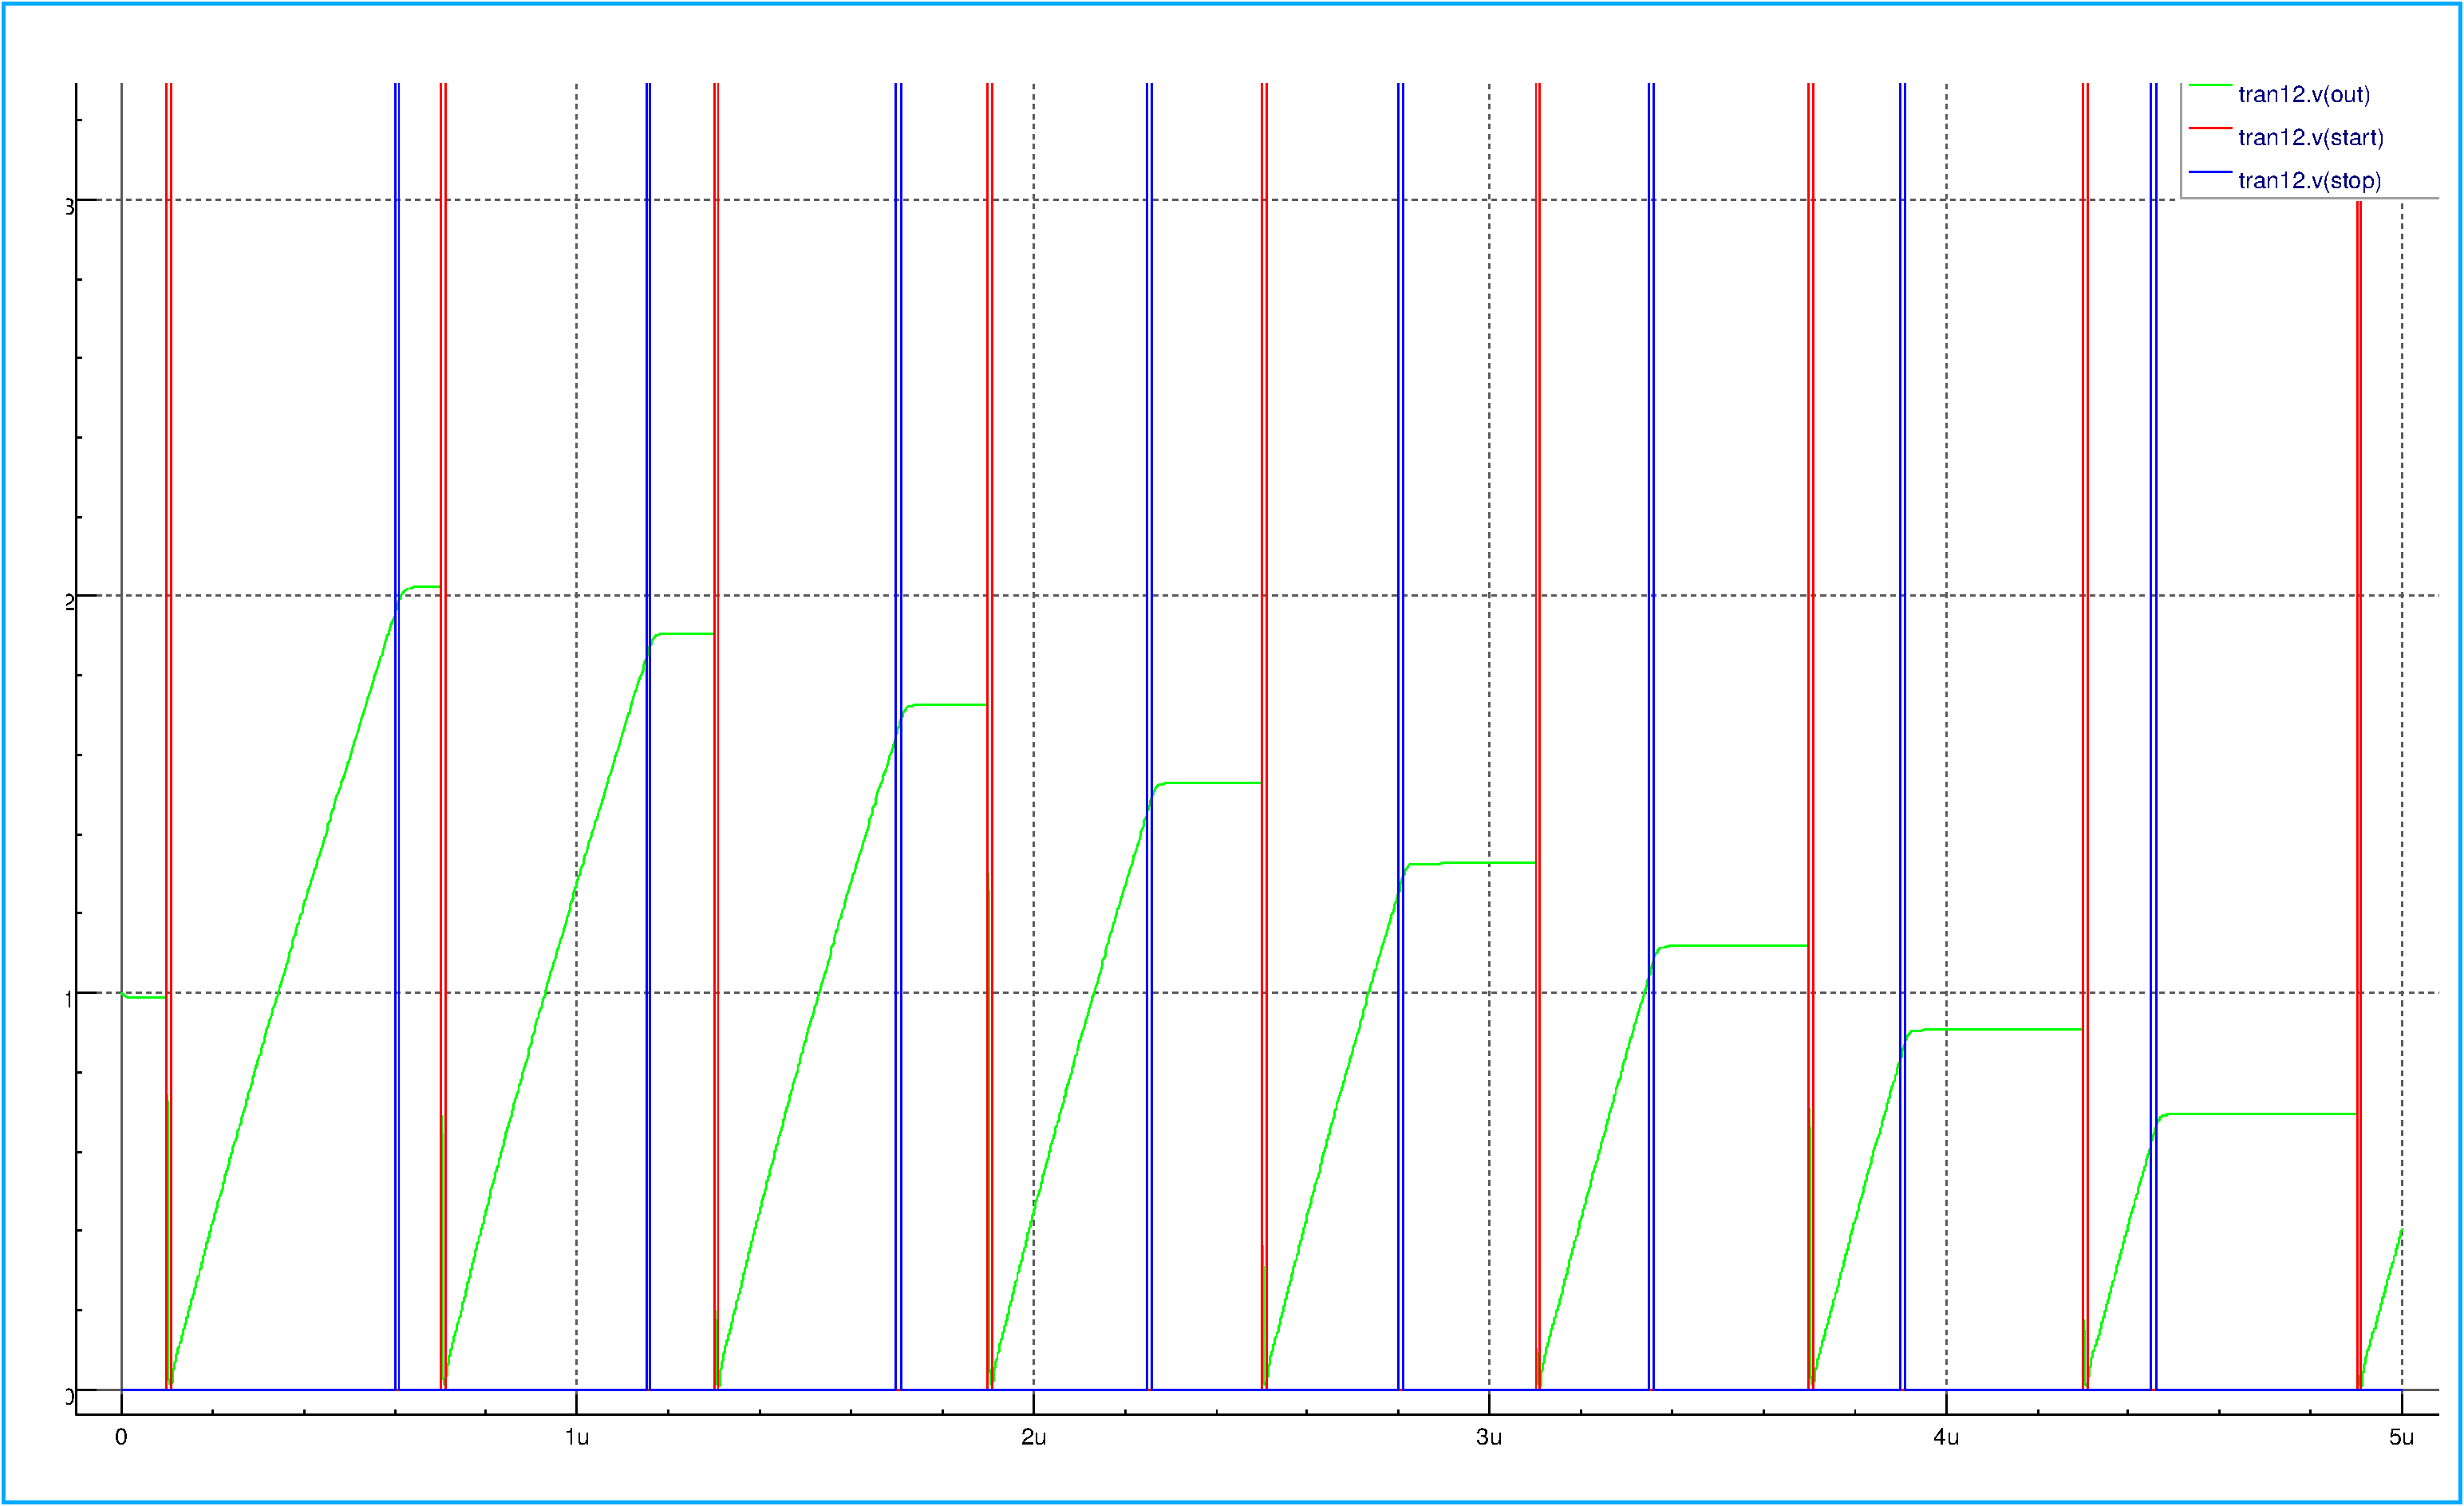
\includegraphics[width=\textwidth]{normalop.pdf}
\label{normal_op}
\caption{Output in normal operation mode}
\end{figure}
\\
As we can see, the output is linear as expected and follows the different variations of the pulses.
To get an idea of the linearity of the circuit, we computed the output characteristic taking different values of delay between the pulses and measuring the output. The delays are sweeped between 25 ns and 500 ns by step of 25 ns.
\newpage
\begin{figure}[!ht]
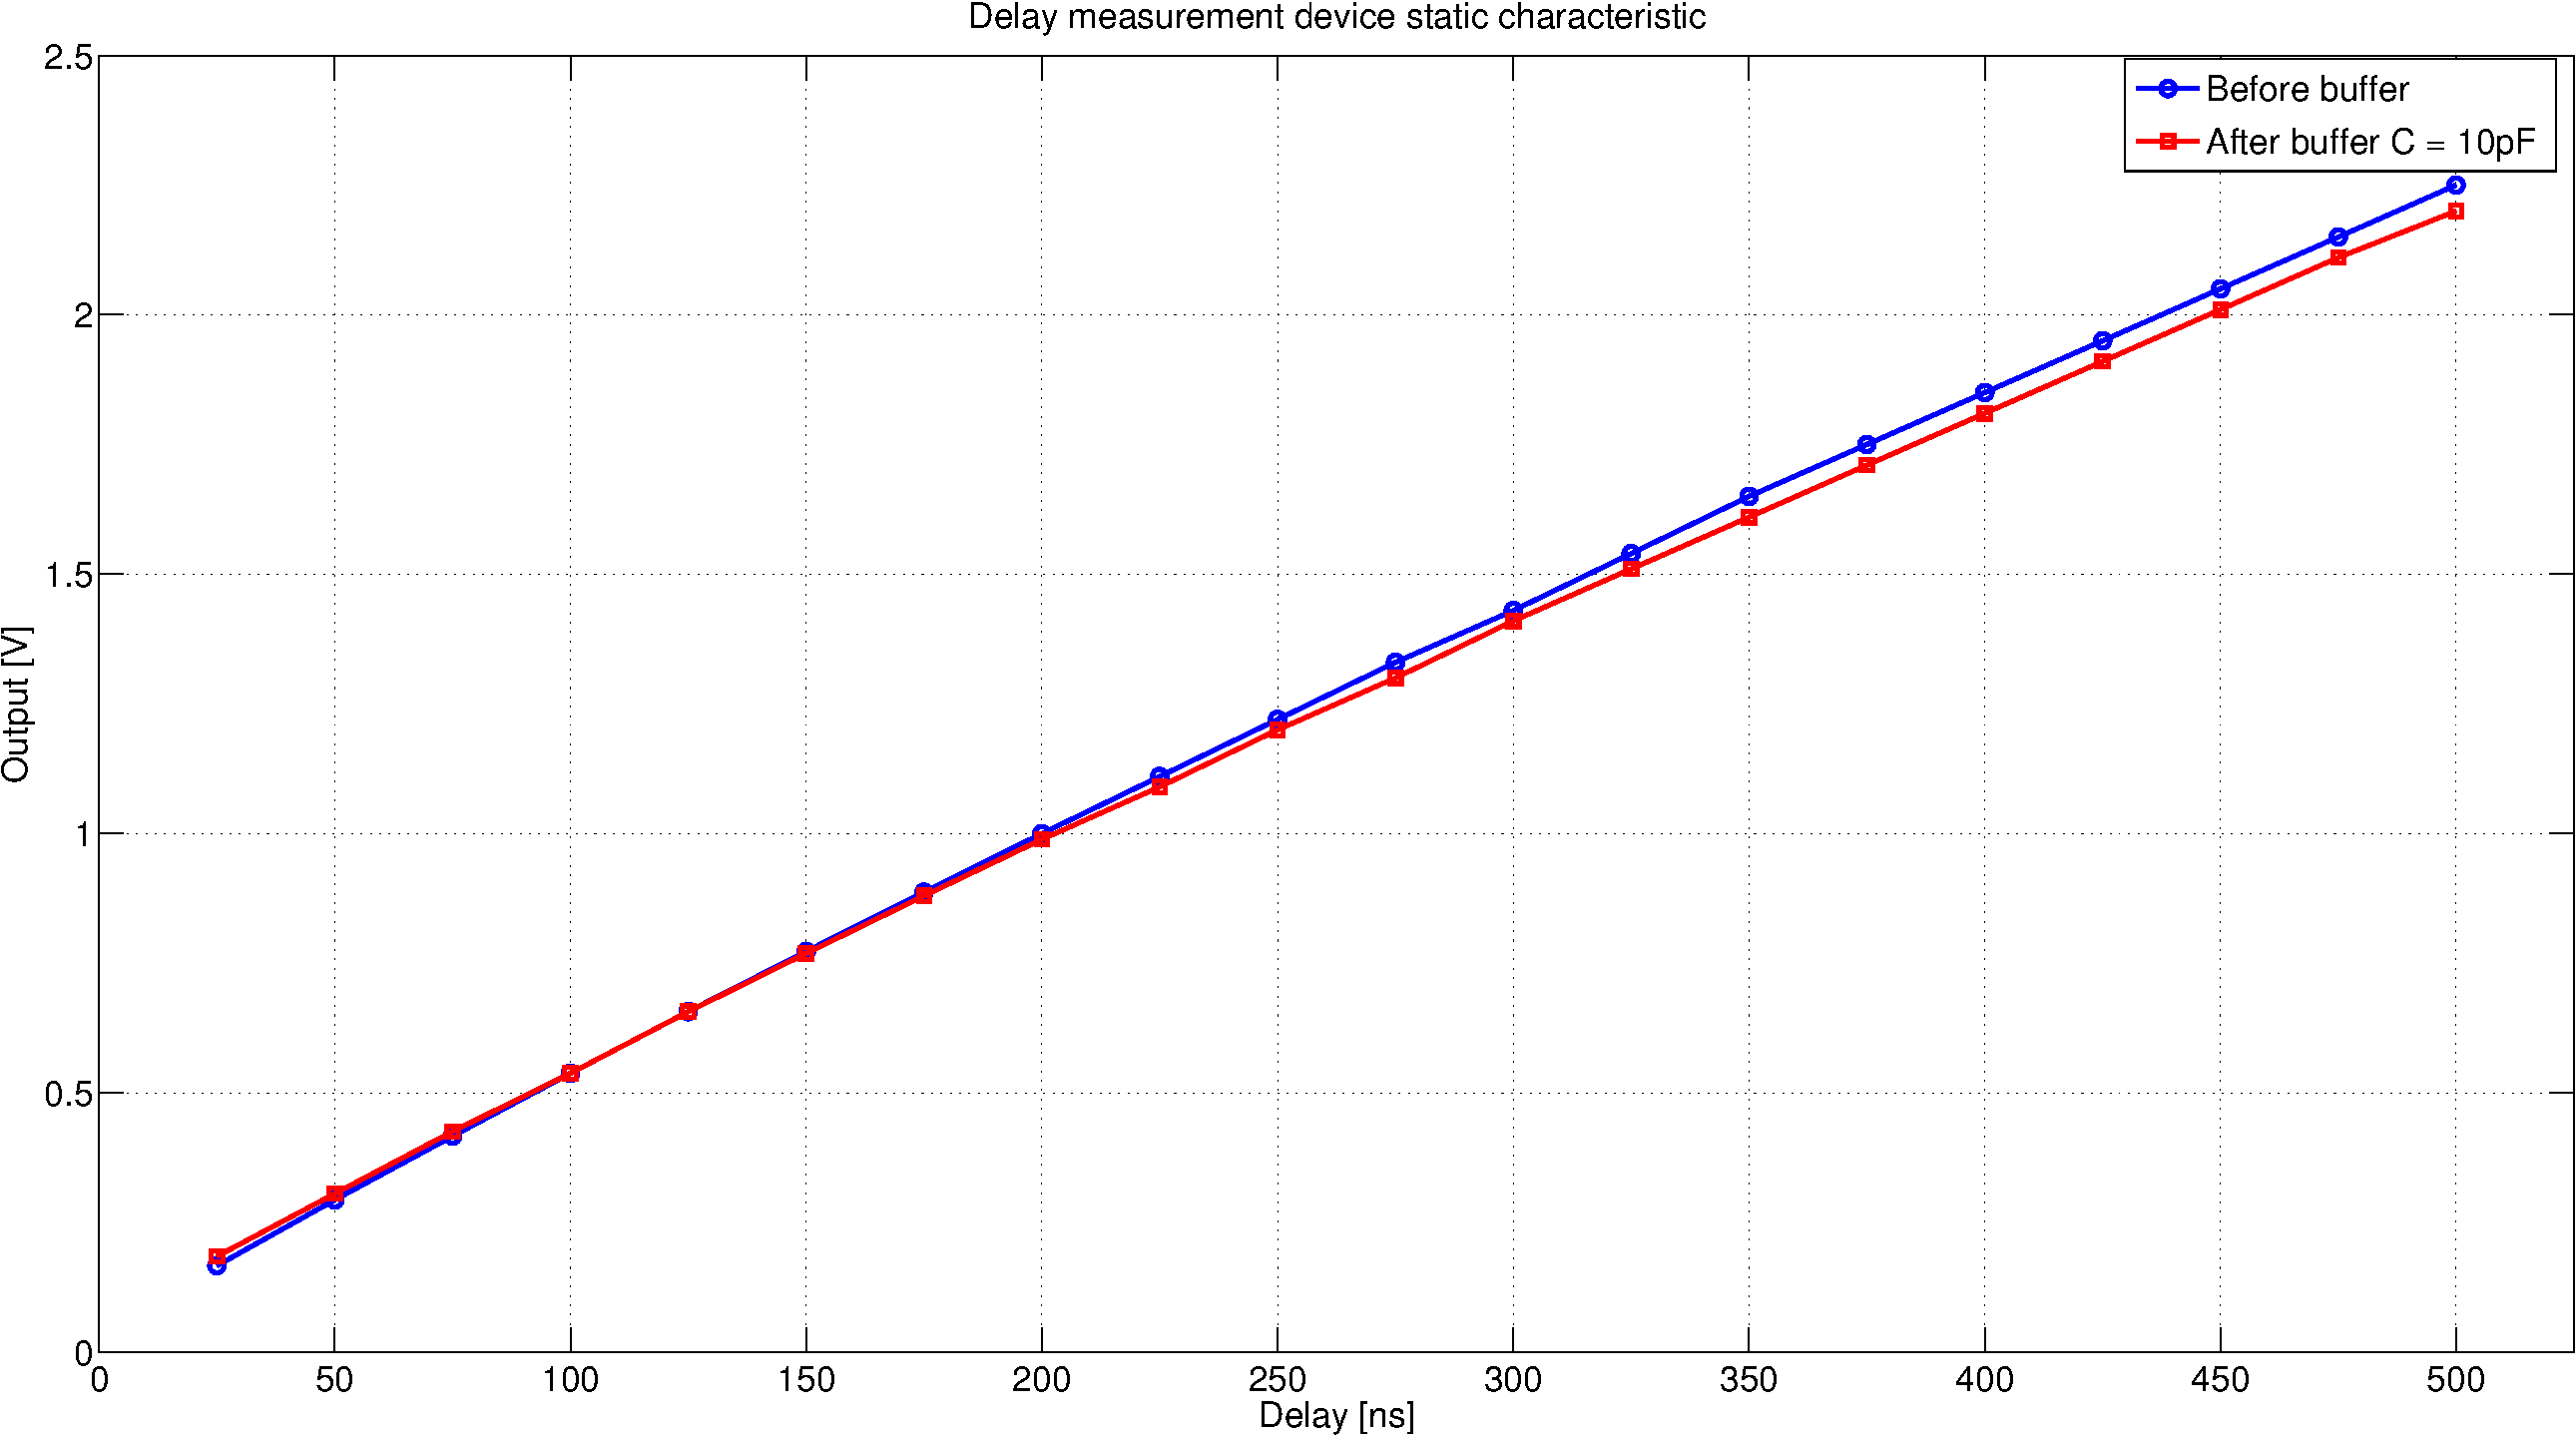
\includegraphics[width=\textwidth]{carac.pdf}
\label{caract}
\caption{Delay measurement}
\end{figure}
As it can be noticed on the Figure\ref{caract} the output characteristic is linear. That goes along with the fact that the circuit is working good even for high delay.
\subsection{Output range}
In order to know the interval in which the circuit is still working as it should be, several pulses have been put each spaced of 70 ns starting at 200 ns. The stopping pulse have been put at 1 us.
\begin{figure}[!ht]
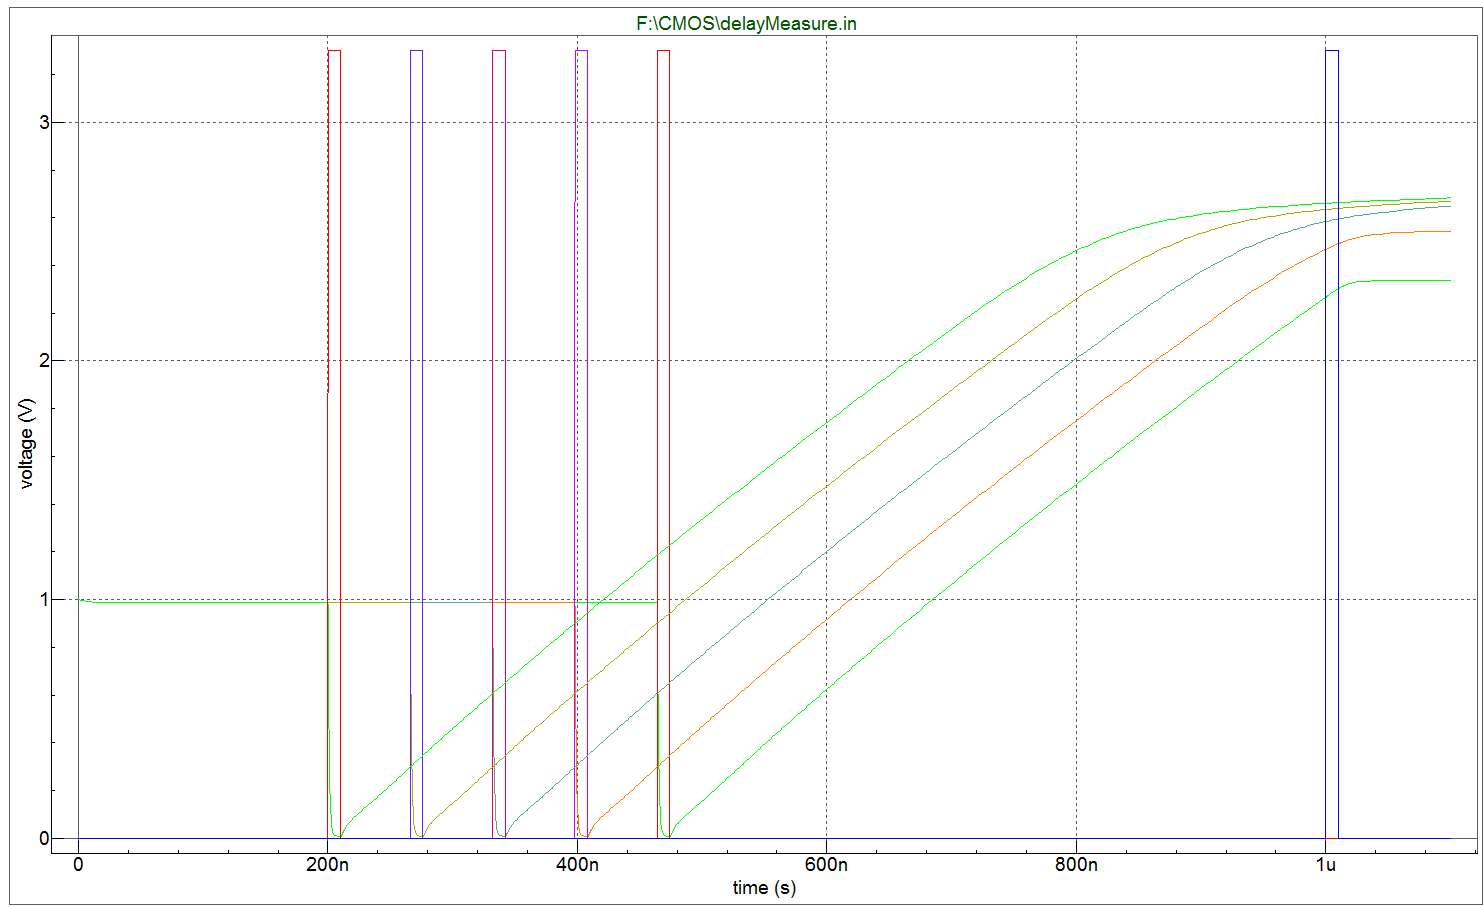
\includegraphics[width=\textwidth]{buffer-satu.png}
\label{buffer_satu}
\caption{Buffer saturating}
\end{figure}

The Figure \ref{buffer_satu} shows clearly that for pulses spaced from 670 ns and above, the output is not linear anymore as the buffer begins to saturate. The output range reached here is approximately equal to 2.4 V. 